\documentclass{beamer}
\usepackage[T1]{fontenc}
\usepackage[utf8]{inputenc}
\usepackage[english]{babel}
\usepackage{amsmath,amsfonts,amssymb}
\usepackage{booktabs}
\usepackage{xcolor}
\usepackage{graphicx}
\usepackage[scaled=0.93]{helvet}
\usetheme{CambridgeUS}
\usecolortheme{beaver}
\setbeamercolor{itemize item}{fg=red}
\setbeamertemplate{itemize items}[square]
\setbeamertemplate{itemize item}[red]
\setbeamertemplate{blocks}[rounded][shadow=false]
\beamertemplatenavigationsymbolsempty

\newcommand{\ket}[1]{\left| #1 \right>} % for Dirac bras
\newcommand{\bra}[1]{\left< #1 \right|} % for Dirac kets
\newcommand{\braket}[2]{\left< #1 \vphantom{#2} \right|
\left. #2 \vphantom{#1} \right>} % for Dirac brackets
\newcommand{\vect}[1]{\boldsymbol{\mathbf{#1}}}


\title[Theory Group Seminar Talk]{\textbf{Diffusion Controlled Reaction Rates over Fluctuating Barriers}}
\author[J.Kolb]{Jakob J. Kolb}
\institute[HU-B: AG Soft Matter Theory]{Helmholtz-Zentrum Berlin\\Soft Matter Theory}
\date{24th January 2014}

\begin{document}


\frame[label=titlepage]{\titlepage}



\section{Introduction}

\frame{
    \begin{minipage}[t]{0.4 \textwidth}
        \begin{figure}[H]
            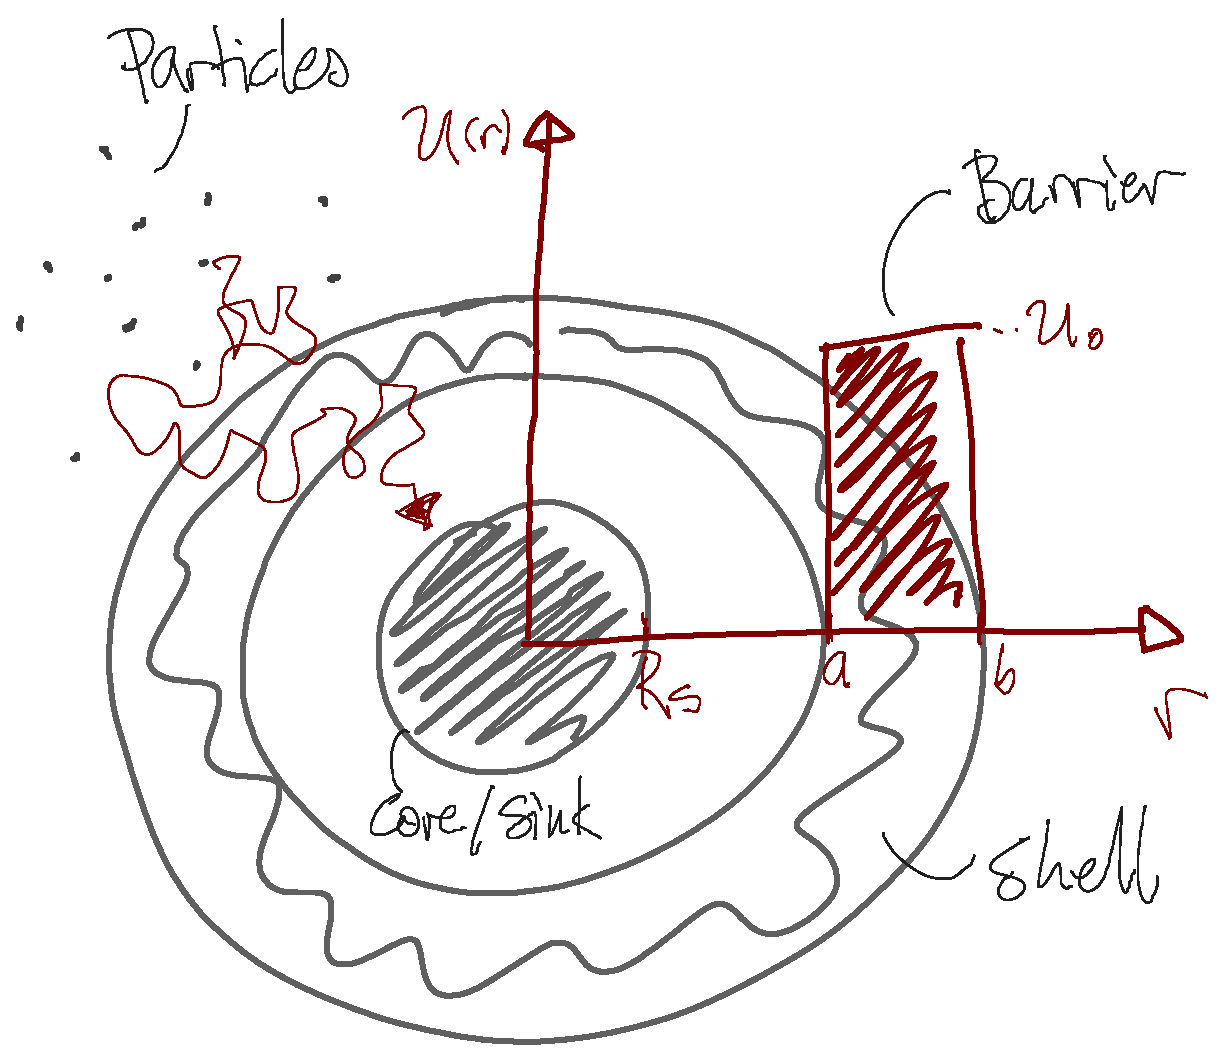
\includegraphics[width = 1 \textwidth]{skizze.eps}
        \end{figure}
    \end{minipage}\vspace{.05 \textwidth}\begin{minipage}[t]{0.55 \textwidth}
        \begin{align*}
            &\frac{d \vec{x}_i}{d t} = -\frac{1}{\gamma}\vec{\nabla}U_i(\vec{x}_i) + \sqrt{2D} \varepsilon(t)\\
            &U_i \in [U_0, \cdots, U_n] \\
            &\frac{d}{d t}\vect{P}_U = \hat{W}\vect{P}_U\\
        & Important \quad property \quad of \quad \hat{W}\\
            &\hat{W}\vect{\rho}^{(eq)} = 0, \quad W_{ij}\rho_{i}^{(eq)} = W_{ji}\rho_{j}^{(eq)}    
        \end{align*}
    \end{minipage}
    The resulting Fokker-Planck equation and boundary conditions are:
    \begin{align}
        &\frac{\partial \vect{\rho}}{\partial t} = \hat{\Gamma}_{FP}\vect{\rho} + \hat{W}\vect{\rho}  \\
        &\hat{\Gamma}_{FP} = {\rm diag}\left[ \vec{\nabla} U_{i}(\vec{r}) \vec{\nabla} + D \vec{\nabla}^{2} \right] \nonumber\\
        &\vect{\rho}(R_s) = 0, \quad \vect{\rho}(r \rightarrow \infty) = \vect{\rho}^{(eq)} \nonumber
        \label{FPE}
    \end{align}

}
\section{Solution}		
\frame{
    Fitting conditions at jump discontinuities of the potential in steady state
    \begin{align}
        &\int_{R_s}^{r}\hat{\Gamma}_{FP}\vect{\rho}(r'){\rm d} r' = - \hat{W} \int_{R_s}^{r} \vect{\rho}(r') {\rm d} r' \nonumber \\
        &\frac{1}{\gamma}\rho_i(r) \vec{\nabla} U_i(r) + D \vec{\nabla} \rho_i(r) = J_i(R_s) - \left\{ \hat{W} \int_{R_s}^{r} \vect{\rho}(r') {\rm d} r' \right\}_{i} \nonumber \\
        &\int_{a-\varepsilon}^{a + \varepsilon} \frac{U_i}{\gamma D}\delta(a-r) + \int_{a-\varepsilon}^{a + \varepsilon} \frac{1}{\rho_i(r)}\nabla \rho_i(r) = \underbrace{\int_{a - \varepsilon}^{a + \varepsilon}\frac{J_i(r)}{\rho_i(r) D} - \int_{a - \varepsilon} ^{a+ \varepsilon} \left\{ \hat{W} \vect{n}(r)\right\}_{i}}_\text{$O(\varepsilon)$} \nonumber 
    \end{align}
    So in the limit of $\varepsilon \rightarrow 0$ we have:
    \begin{equation}
        \vect{\rho}^{I} =  {\rm diag}\left[\exp\left\{\frac{U_i}{K_B T} \right\}\right] \vect{\rho}^{II}
    \end{equation}
    }
\frame{
for $r \ne a,b$ and steady state:
\begin{equation*}
    0 = D \vec{\nabla}^{2} \vect{\rho} + \hat{W} \vect{\rho}
\end{equation*}
Goal: decoupling of equations i.e. orthonalization of $\hat{W}$.
\begin{equation*}
    \hat{T}_{i,j} = \delta_{i,j}\frac{1}{\sqrt{\rho^{(eq)}_{i}}}; \quad \hat{T}^{-1}\hat{W}\hat{T} = \hat{S}
\end{equation*}
since $\hat{S}$ is symetric, there is an orthononal transformation $\hat{D}$ such that:
\begin{equation*}
    \hat{D}^{\dagger}\hat{S}\hat{D} = -\hat{d}; \quad \hat{d} = {\rm diag}\left[|\lambda_i|\right], \quad \lambda_1 = 0, \lambda_{i>0}<0
\end{equation*}
thus the FPE becomes independent for different states of $U$
\begin{equation}
    0 = D \vec{\nabla}^{2}\tilde{\vect{\rho}} - \hat{d} \tilde{\vect{\rho}}, \quad \tilde{\vect{\rho}} = \hat{L} \vect{\rho} = \hat{T}\hat{D}\vect{\rho}
\end{equation}
}
\frame{
Solutions for this equation are:
\begin{align}
    &\tilde{\rho}_{1}(r) = C_{1,1} + C_{1,2}\frac{1}{r} \nonumber \\
    &\tilde{\rho}_{i \ne 1}(r) = C_{i,1} \exp \left[-r \sqrt{\frac{|\lambda_i|}{D}} \right]+C_{i,2} \exp \left[r \sqrt{\frac{|\lambda_i|}{D}} \right]
\end{align}
Transformed boundary and fit conditions:
\begin{align*}
    \hat{L}^{-1}\tilde{\vect{\rho}}^{(I)}(R_s) &= \tilde{\vect{\rho}}^{(I)}(R_s) = 0 \nonumber \\
    \tilde{\vect{\rho}}(r \rightarrow \infty) &= \hat{L}^{-1} \tilde{\vect{\rho}}^{(eq)} = (1,0,\cdots,0)
\end{align*}
and
\begin{align*}
    \tilde{\vect{\rho}}^{(I)}(a) &= \hat{L}^{-1}\mathrm{diag}[\exp(\frac{U_i}{K_B T})]\hat{L} \tilde{\vect{\rho}}^{(II)}(a), \\ \nonumber
    \tilde{\vect{\rho} '}^{(I)}(a) &= \tilde{\vect{\rho} '}^{(II)}(a), \\ \nonumber
    \tilde{\vect{\rho}}^{(III)}(b) &= \hat{L}^{-1}\mathrm{diag}[\exp(\frac{U_i}{K_B T})]\hat{L} \tilde{\vect{\rho}}^{(II)}(b), \\ \nonumber
    \tilde{\vect{\rho} '}^{(III)}(b) &= \tilde{\vect{\rho} '}^{(II)}(b)
\end{align*}
}
\frame{
Now, lets calculate some rates!
\begin{align}
    K = \int_{\partial Sink} \vec{J} {\rm d} \vec{A} &= 4 \pi D R_{s}^{2} \left. \frac{\partial}{\partial r} \right|_{R_s} \sum_i \rho_{i}(r) \nonumber \\
    & = 4 \pi D R_{s}^{2} \left. \frac{\partial}{ \partial r } \right|_{R_s} \sum_i \left\{ \hat{L} \tilde{\vect{\rho}}(r) \right\}_i
\end{align}
\begin{itemize}
    \item numeric calculation of $C_{i,j}$ coefficients for fitting and boundary conditions
    \item plot analytic solution for reaction rates
    \item comparison with results from BD simulations
\end{itemize}

}
\section{Results}
\frame{
	\begin{minipage}[t]{0.5 \textwidth}
        \begin{figure}[H]
            \includegraphics[width = 1 \textwidth]{interpol.eps}
            \caption{Limiting cases and analytic solution for reaction rate}
        \end{figure}
    \end{minipage}\vspace{.05 \textwidth}\begin{minipage}[t]{0.5 \textwidth}
        \begin{figure}[H]
            \includegraphics[width = 1 \textwidth]{det.eps}
            \caption{Determinant of boundary condition matrix}
        \end{figure}
    \end{minipage}
}
\frame{
	\begin{minipage}[t]{0.6 \textwidth}
        \begin{figure}[H]
            \includegraphics[width = 1 \textwidth]{u+1.eps}
            \caption{Reaction rates for different barrier width}
        \end{figure}
    \end{minipage}\vspace{.05 \textwidth}\begin{minipage}[t]{0.4 \textwidth}
        \begin{figure}[H]
            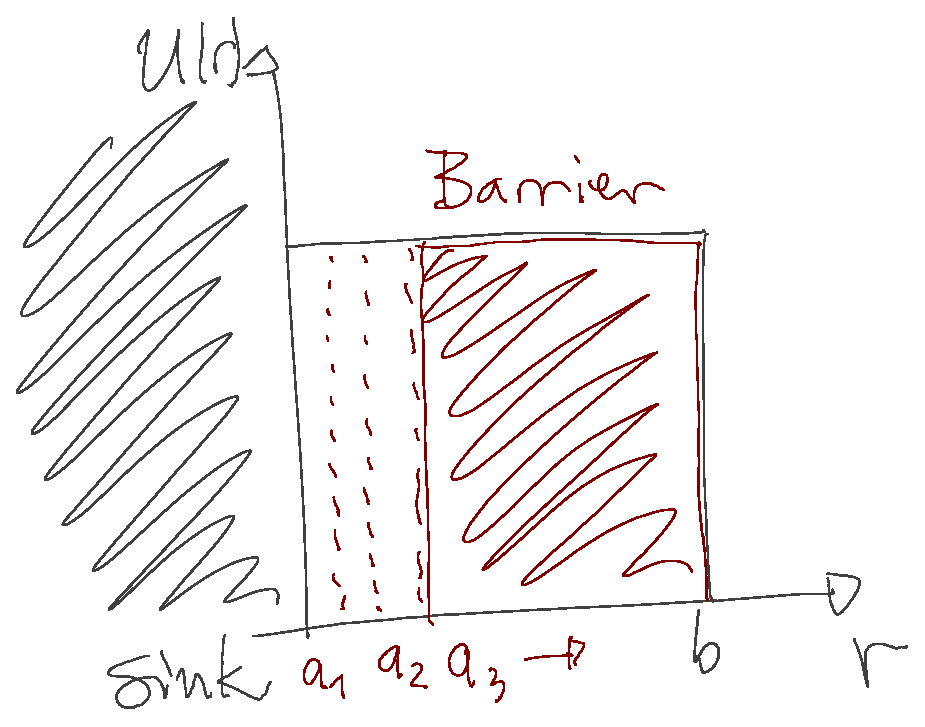
\includegraphics[width = 1 \textwidth]{skizze2.eps}
            \caption{Sketch of potential barrier}
        \end{figure}
    \end{minipage}
}
\frame{
	\begin{minipage}[t]{0.6 \textwidth}
        \begin{figure}[H]
            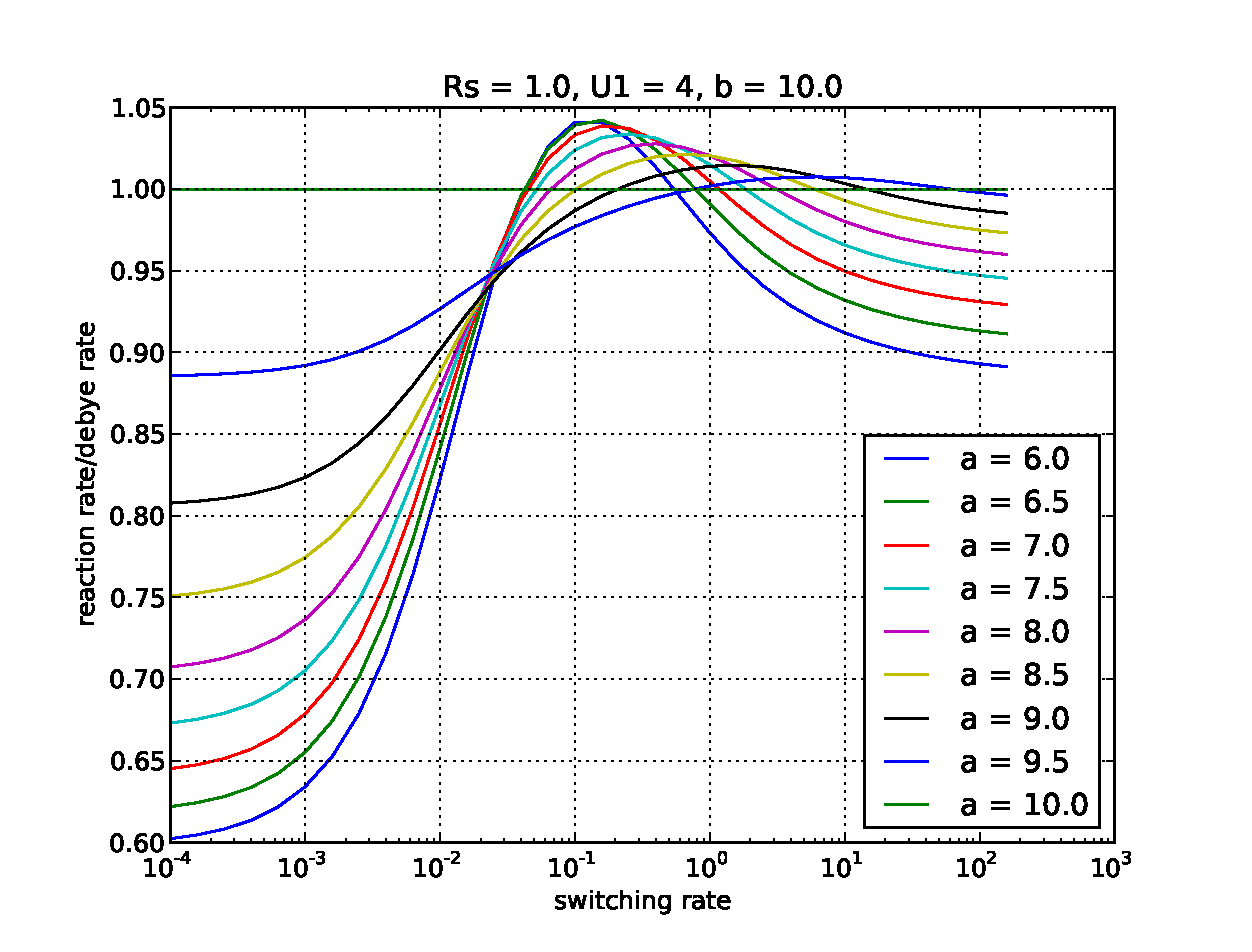
\includegraphics[width = 1 \textwidth]{u+2.eps}
            \caption{Reaction rates for different barrier width}
        \end{figure}
    \end{minipage}\vspace{.05 \textwidth}\begin{minipage}[t]{0.4 \textwidth}
        \begin{figure}[H]
            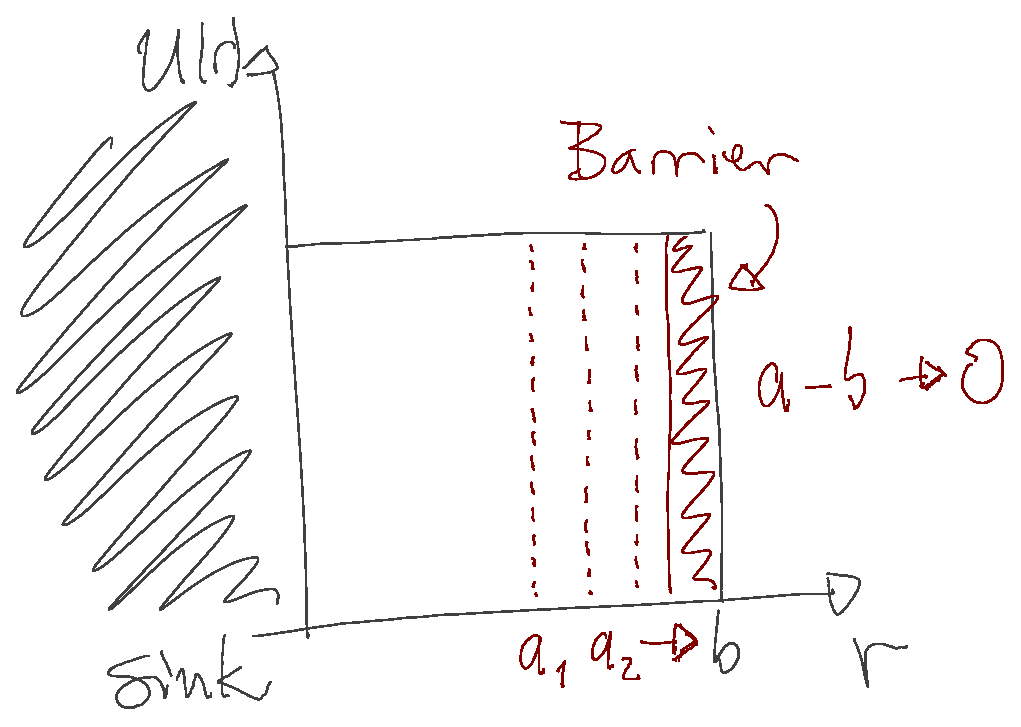
\includegraphics[width = 1 \textwidth]{skizze3.eps}
            \caption{Sketch of potential barrier}
        \end{figure}
    \end{minipage}
    \begin{itemize}
        \item \textbf{System shows resonant activation!}
    \end{itemize}
}
\section{Simulations}
\frame{
    \begin{minipage}[t]{0.4 \textwidth}
        \begin{figure}[H]
            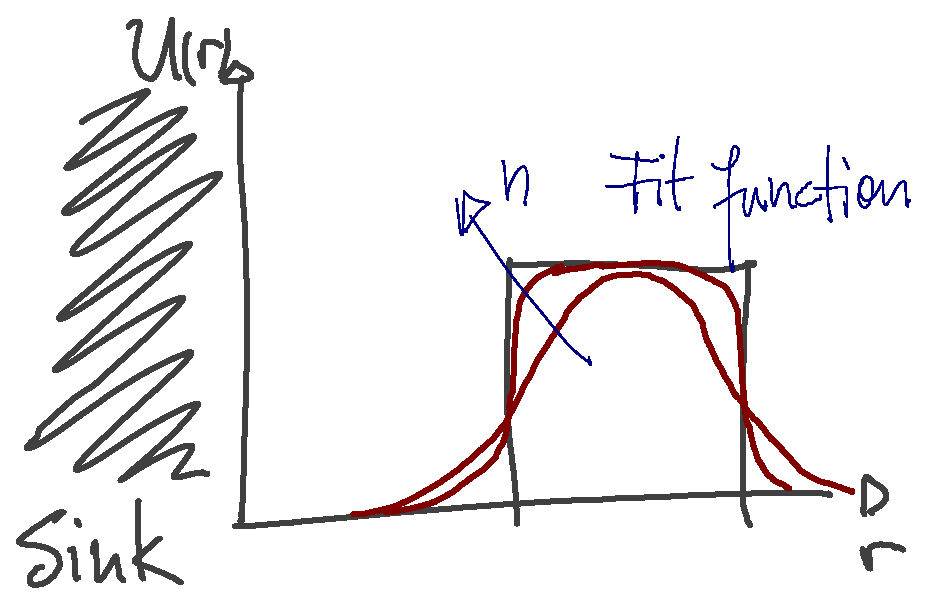
\includegraphics[width = 1 \textwidth]{skizze4.eps}
        \end{figure}
        \begin{figure}[H]
            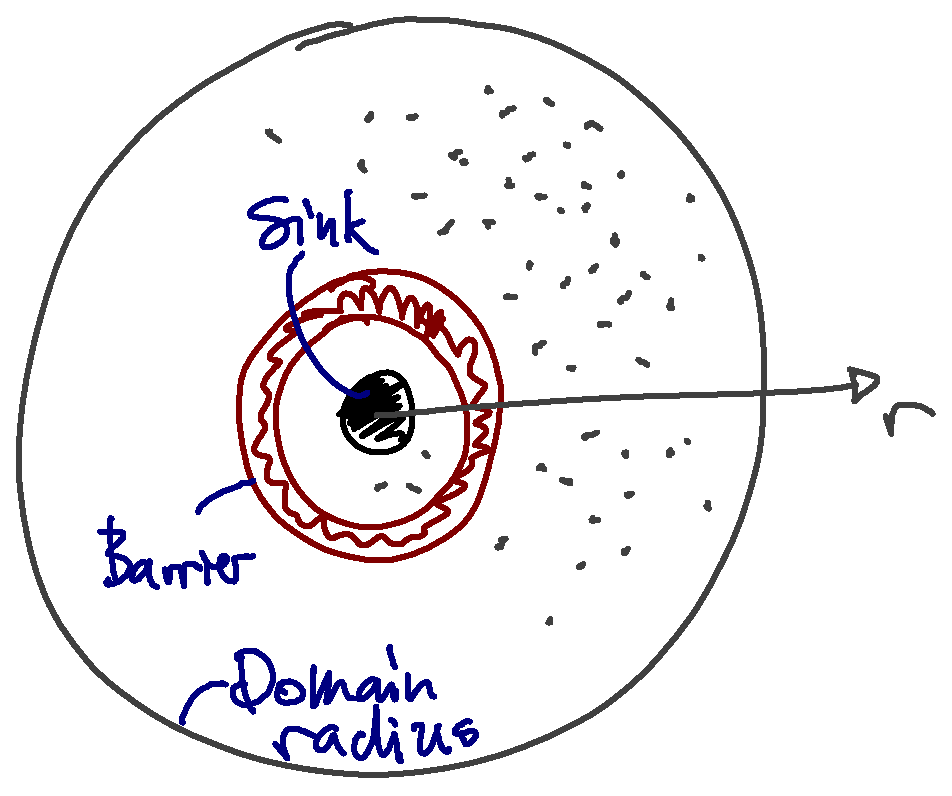
\includegraphics[width = 0.8 \textwidth]{skizze5.eps}
        \end{figure}
        \end{minipage}\hspace{.09 \textwidth}\begin{minipage}[t]{.5 \textwidth}
            Brownian dynamics with approximate boxcar potential barrier:
            \begin{align*}
                &x(t + \Delta t) = x(t) + \frac{1}{\gamma}\vec{\nabla}U(x(t)) \Delta t \\
                &\qquad+ \sqrt{2 D \Delta t} R(t) \\
                &U(r) = \frac{U_0}{\left( \frac{2}{b}(r - a) \right)^{2n}+1} \\
                &K = E\left( \frac{\Delta N}{\Delta t} \right)
            \end{align*}
            Spherical simulation domain to retain symmetry of solution.
        \end{minipage}
}
\frame{
    \frametitle{Analytic solution vs. simulated density profile}
    \begin{minipage}[t]{.5 \textwidth}
        \begin{figure}
            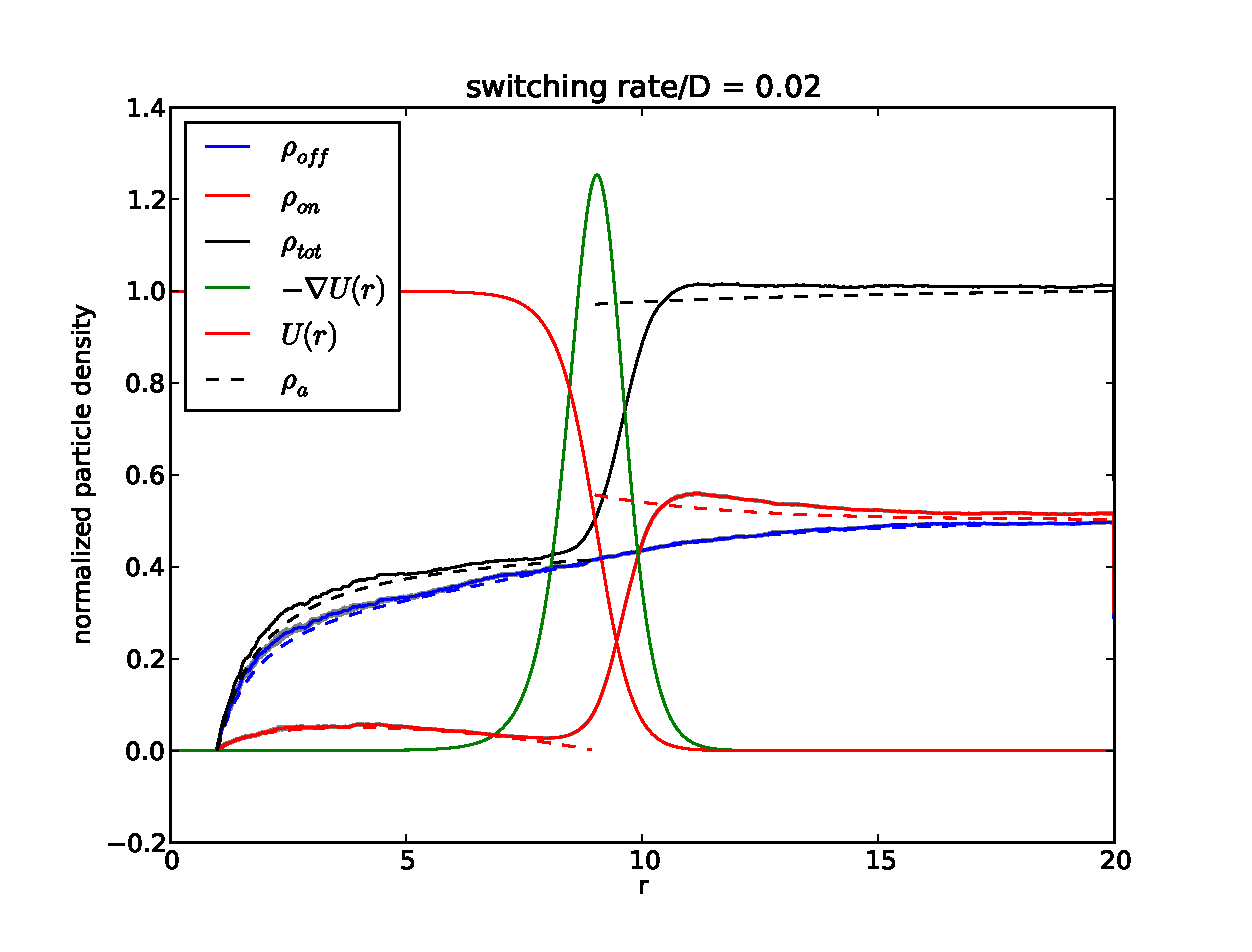
\includegraphics[width = 1 \textwidth]{rho002.eps}
        \end{figure}
    \end{minipage}\begin{minipage}[t]{.5 \textwidth}
        \begin{figure}
            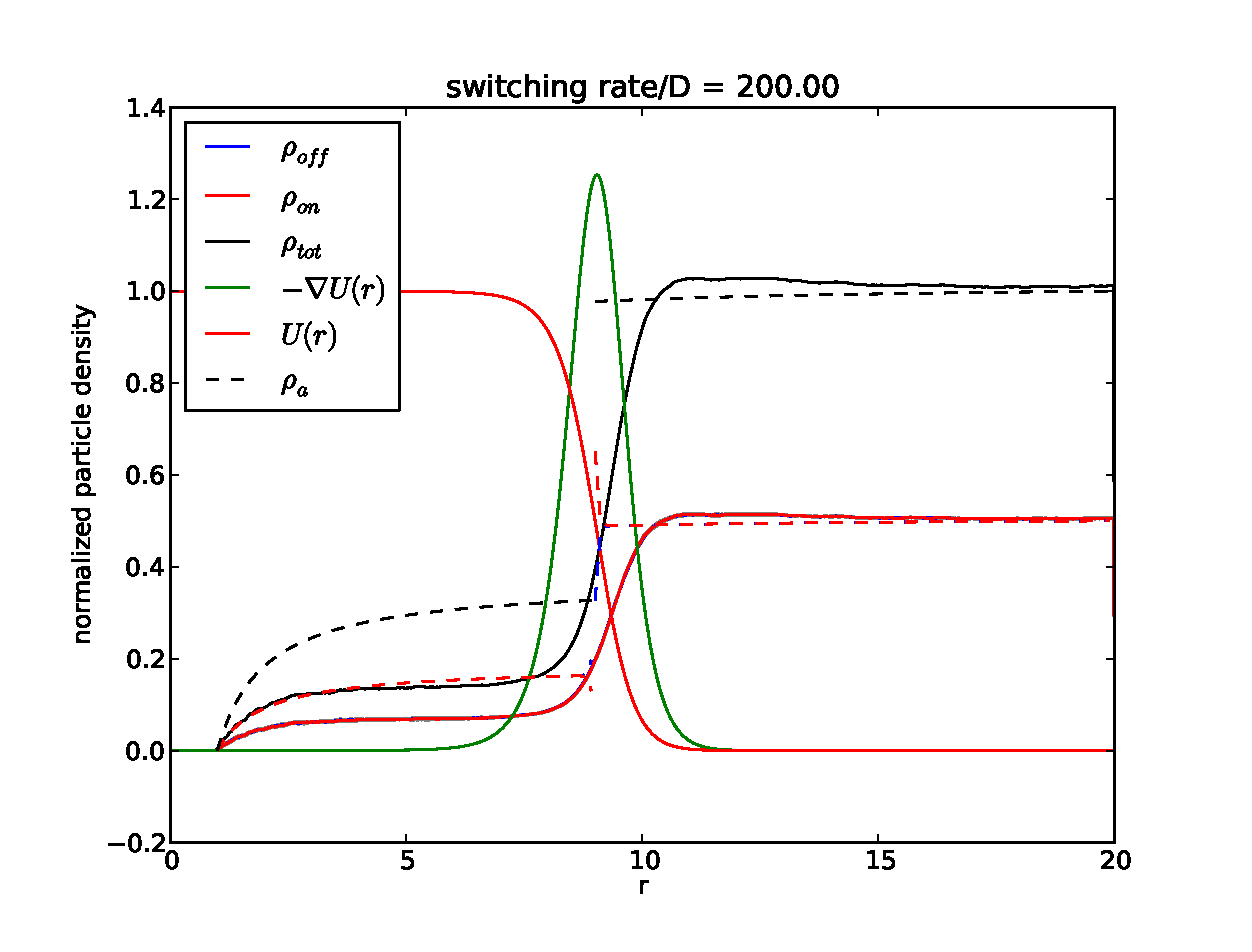
\includegraphics[width = 1 \textwidth]{rho200.eps}
        \end{figure}
    \end{minipage}

We see: Approximation with smooth potential does not work too well.

}

\frame{
    \frametitle{Analytic solution vs. simulated reaction rates}
    \begin{minipage}[c]{0.6 \textwidth}
        \begin{figure}[H]
            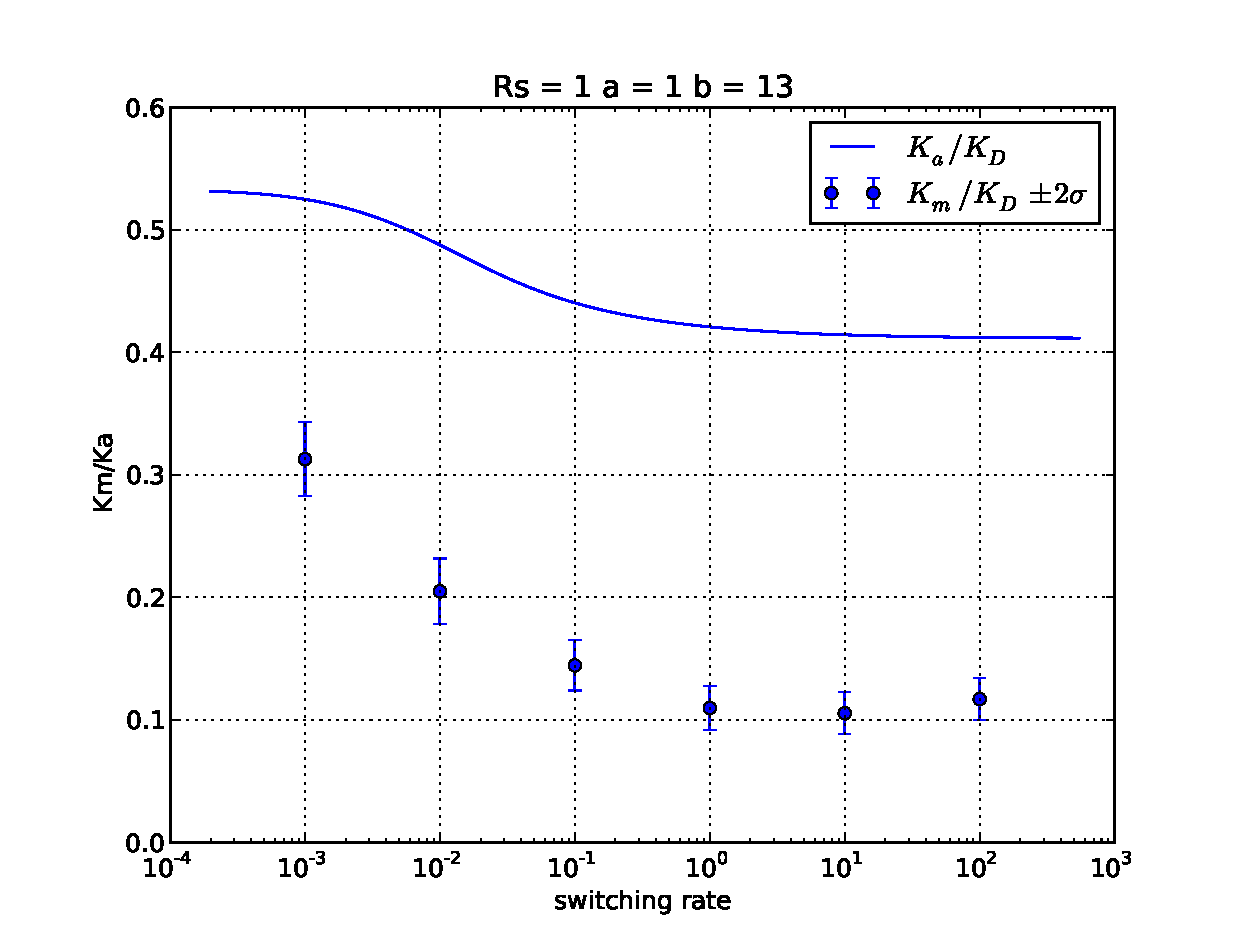
\includegraphics[width = 1 \textwidth]{comp.eps}
        \end{figure}
    \end{minipage}\begin{minipage}[t]{0.4 \textwidth}
    \begin{itemize}
        \item qualitative behaviour matches
        \item quantitatively wrong
    \end{itemize}
    \end{minipage}
}
\frame{
    \frametitle{Convergence for increasing potential steepness?}
    \begin{minipage}{0.6 \textwidth}
    \begin{figure}[H]
        \only<1>{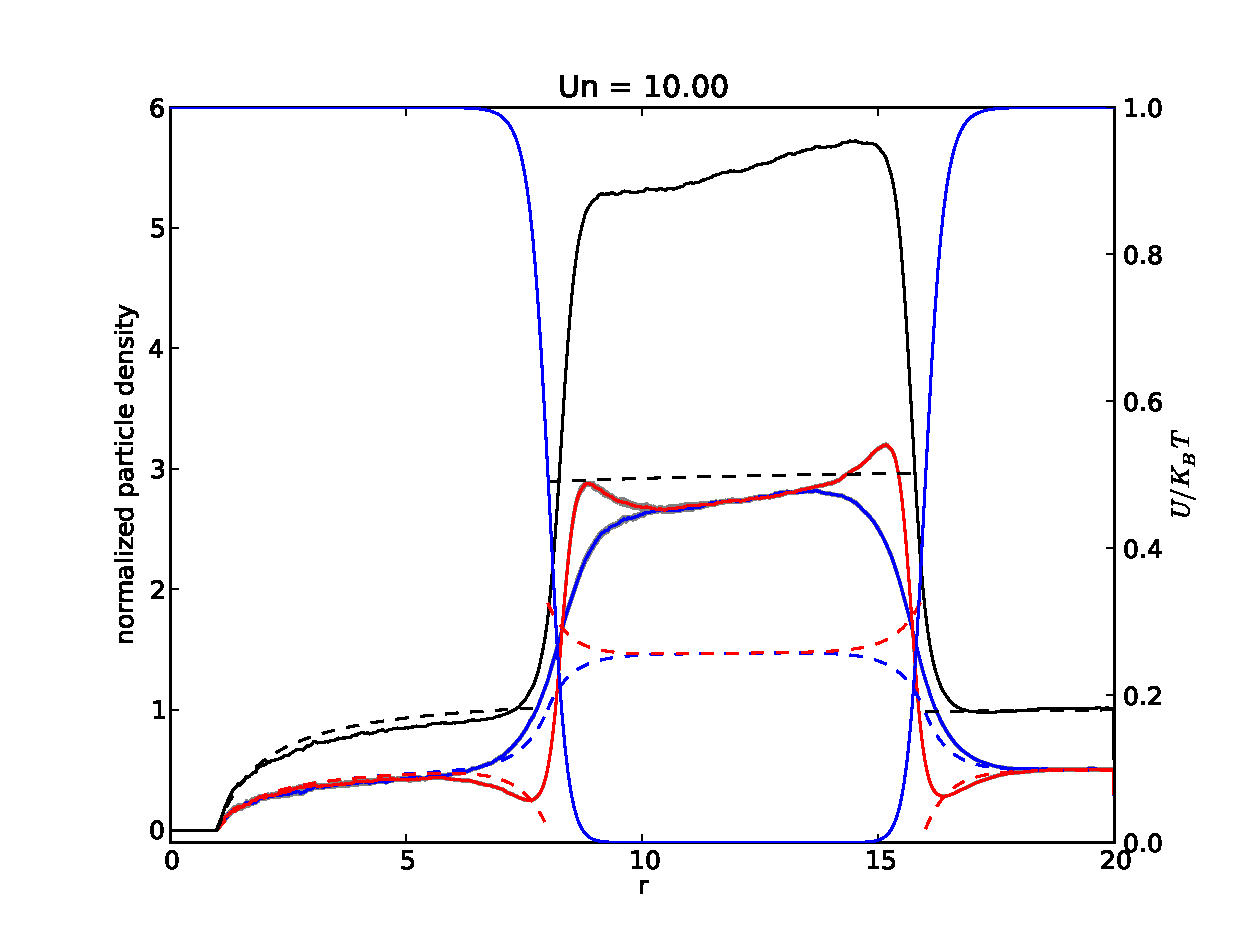
\includegraphics[width = 1 \textwidth]{Un10.eps}}
           \only<2>{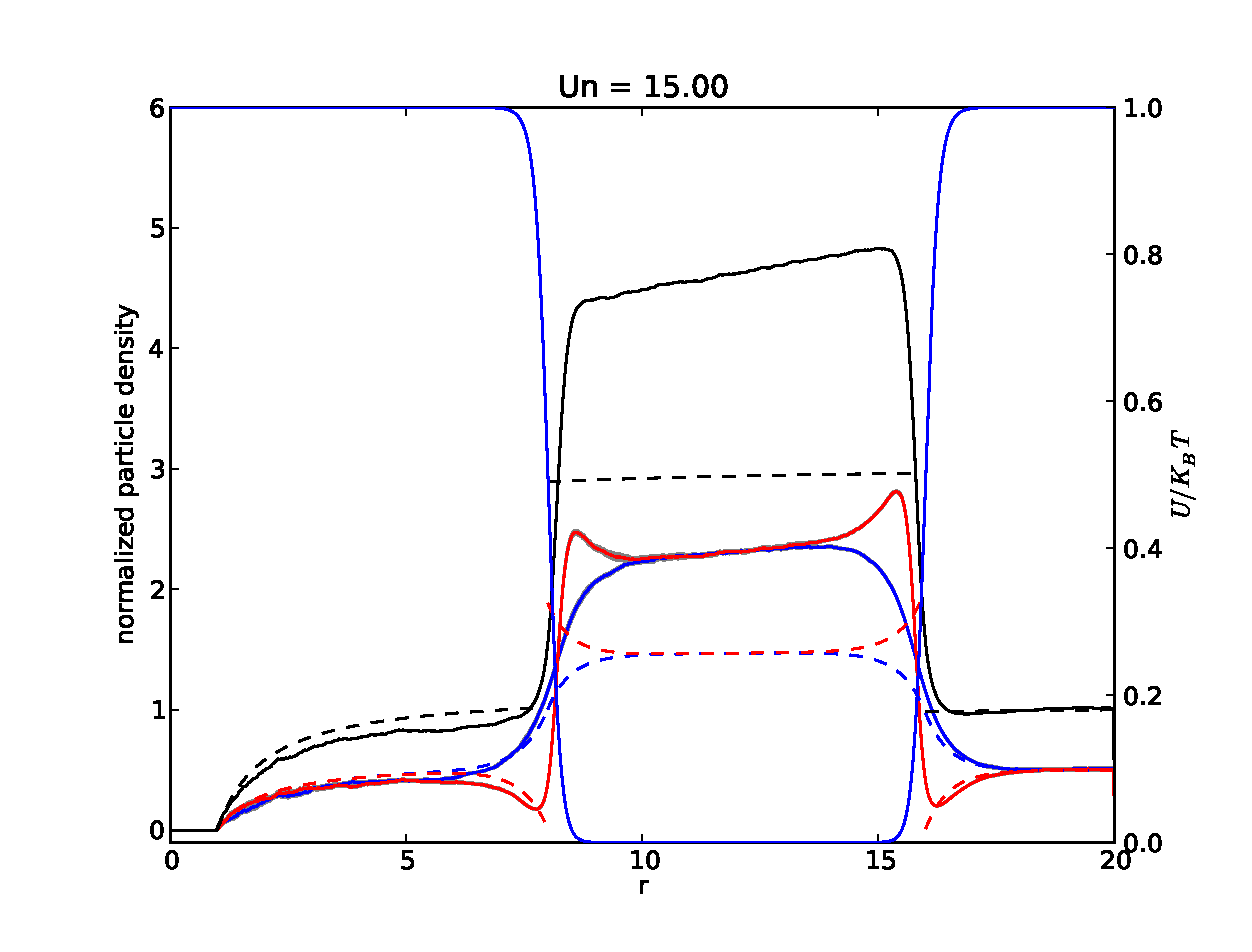
\includegraphics[width = 1 \textwidth]{Un15.eps}}
           \only<3>{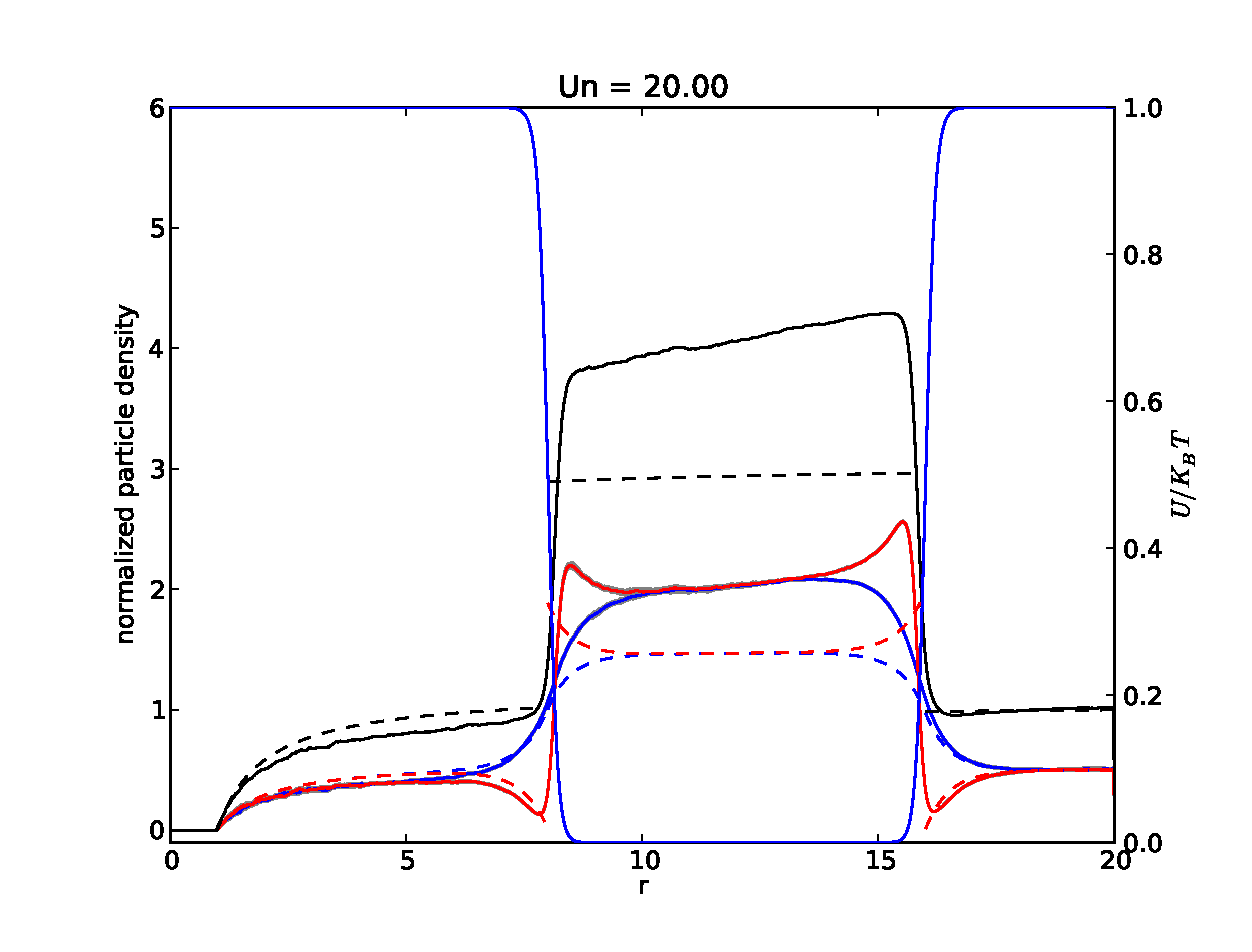
\includegraphics[width = 1 \textwidth]{Un20.eps}}
           \only<4>{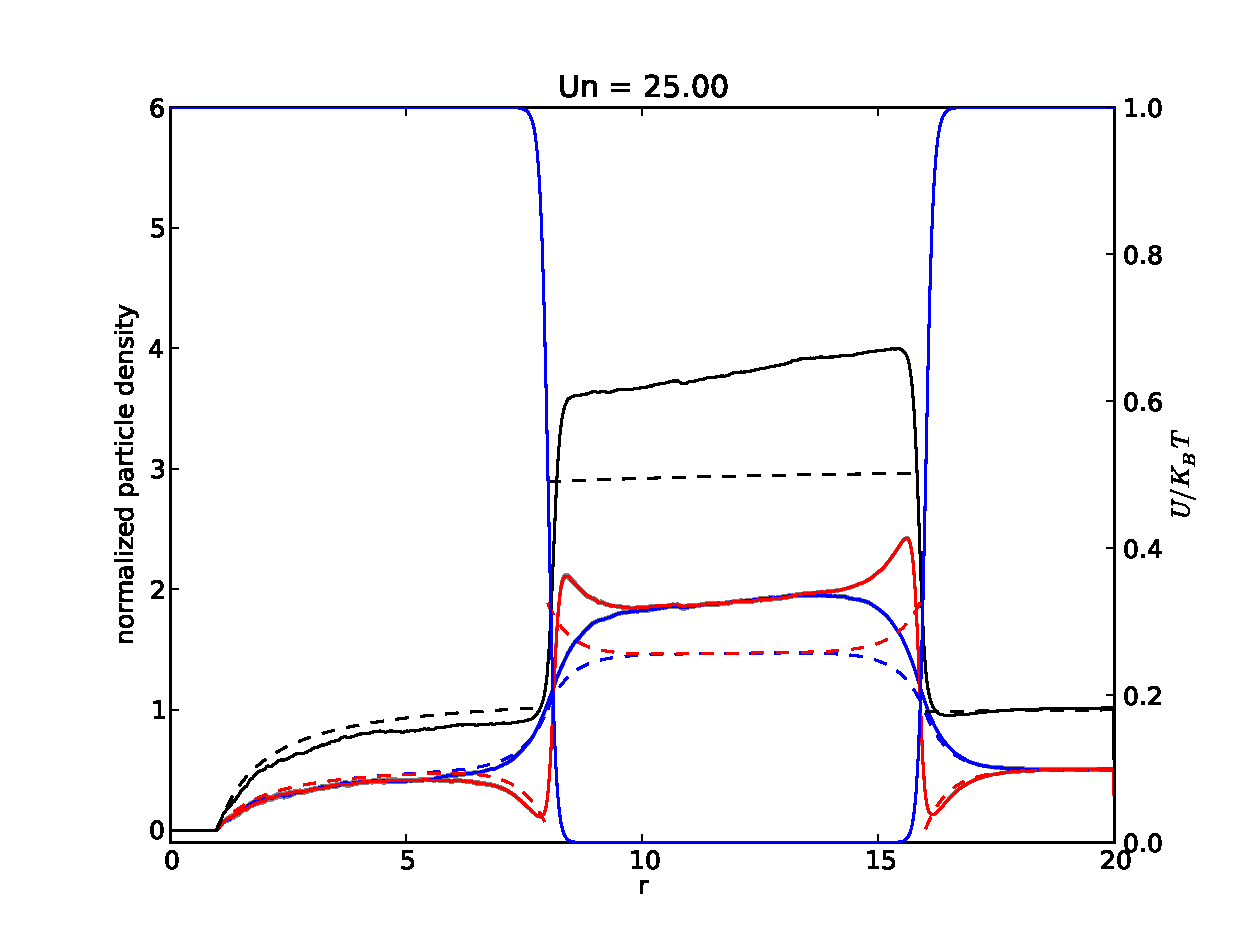
\includegraphics[width = 1 \textwidth]{Un25.eps}}
           \only<5>{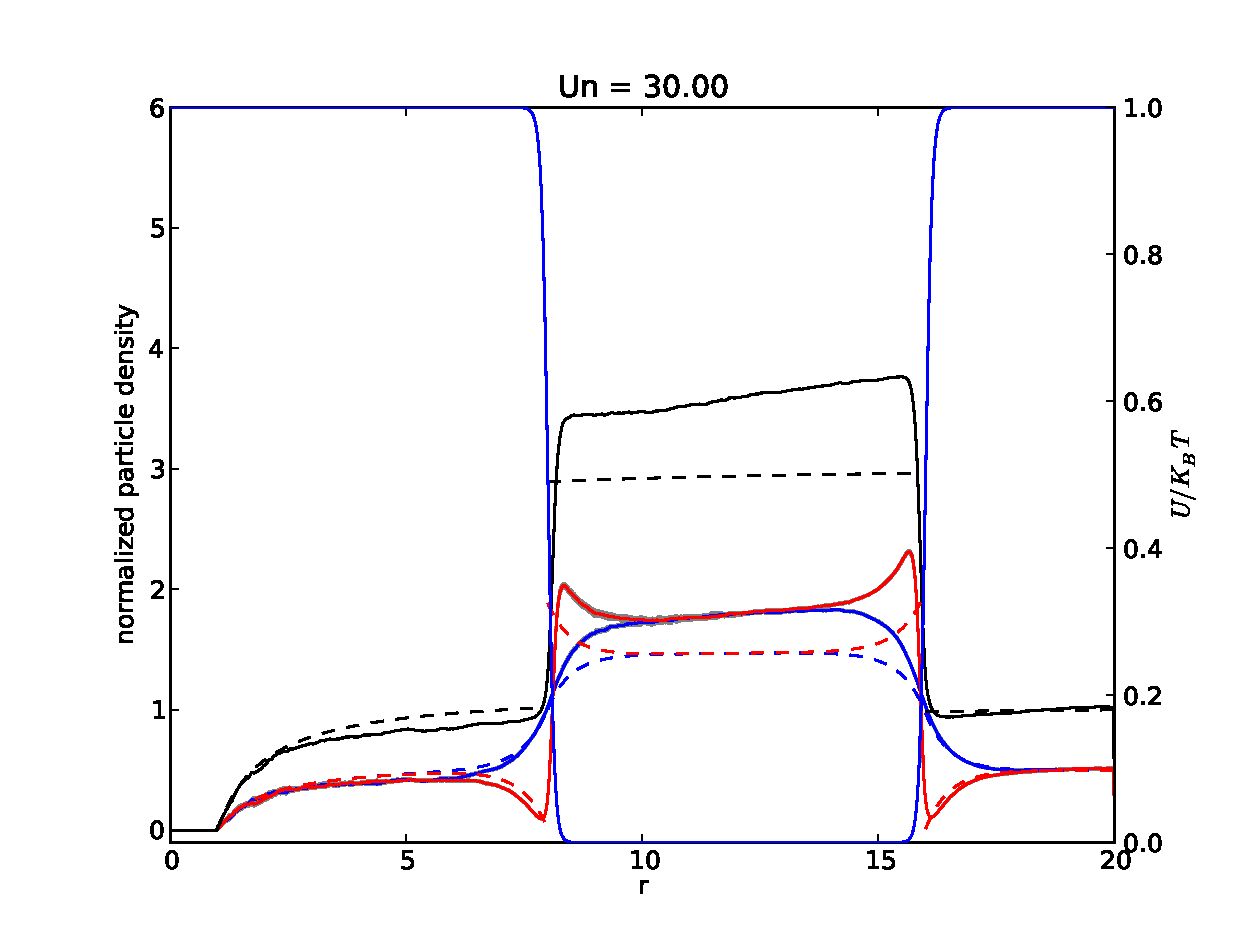
\includegraphics[width = 1 \textwidth]{Un30.eps}}
           \only<6>{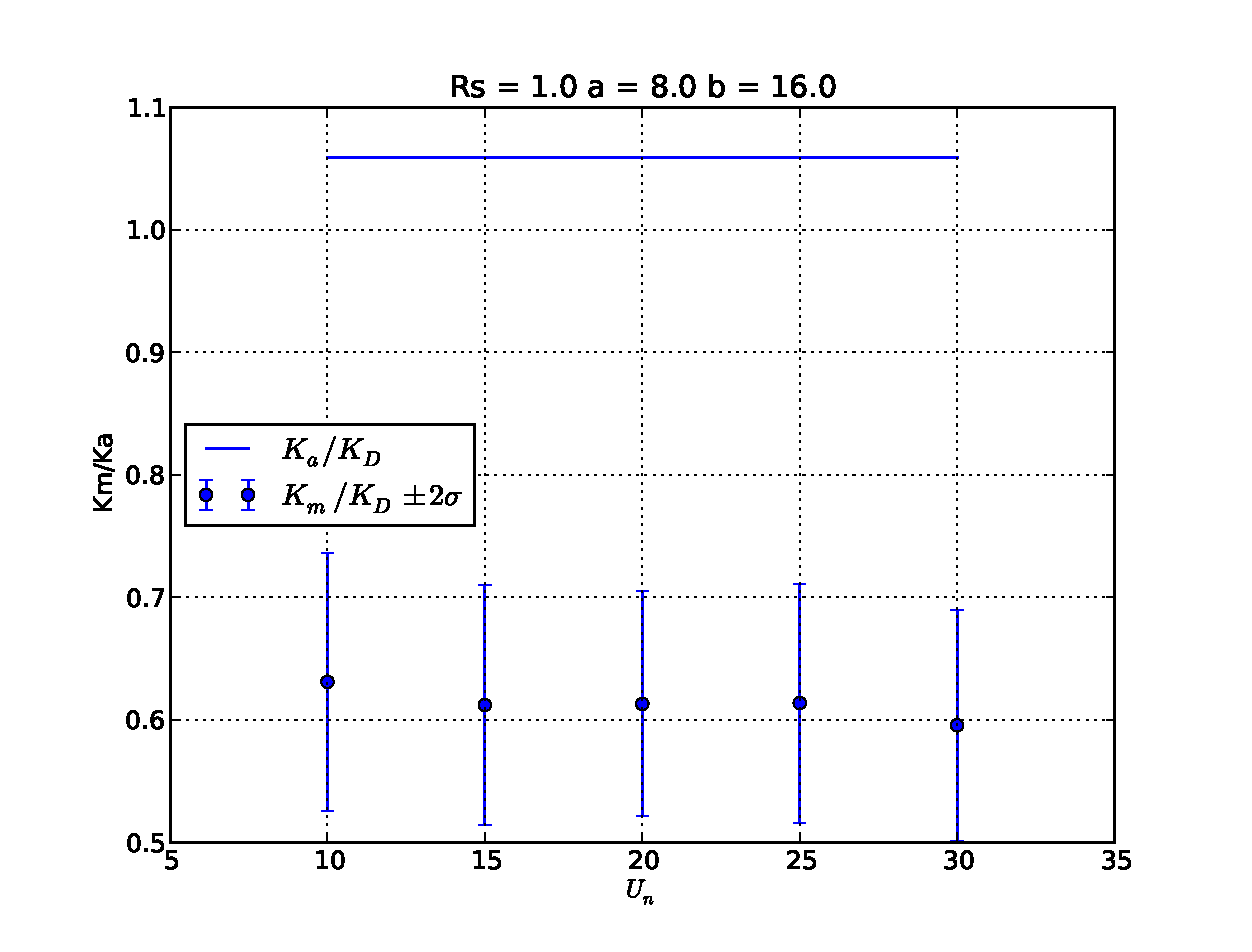
\includegraphics[width = 1 \textwidth]{Un-rates.eps}}
        \end{figure}
    \end{minipage}\begin{minipage}[t]{0.38 \textwidth}
    \begin{itemize}
        \item convergence in density profiles
        \item count for absorbed particles still buggy
    \end{itemize}
    \end{minipage}
}

\section{Summary}
\frame{
    \frametitle{\textbf{Summary}}
    \begin{itemize}
        \item Analytic solution for boxcar like potential barrier possible,
        \item numeric calculation breaks down in limiting cases,
        \item approximation of boxcar potential in BD causes problems
        \item but qualitative behaviour matches well.
    \end{itemize}
}
\section{To Do}
\frame{
    \frametitle{\textbf{To Do}}
    \begin{itemize}
        \item find limiting behaviour for very fast/slow potential fluctuations,
        \item find limiting behaviour for very attractive/repulsive barrier,
        \item are approximate solutions for smooth potentials possible?
        \item Some work to do to converge simulation and analytic solution
    \end{itemize}
}
\end{document}


